\section{Question I: Revisiting HW4 Bank Classification with New Tools (for dataset A)}
\subsection{Data preprocessing}
For this part of the assignment, the dataset had to be analyzed first as part of the preprocessing step to get the structure ,detect issues such as missing values and outliers. The bank marketing data(bank-additional.csv) has 4119 observations and 21 features.There was found to be 1230 unknowns in the categorical features of the dataset. Features that had unknowns were checked and there was found to be six features: job,marital,education,default,housing,loan that had unknowns( 0.96 ,0.3 ,4.1,  19.5, 2.6)\% respectively.Removing rows with missing values can be too limiting on some predictive modeling problems. The proportion of the unknown's is sparse, the mode of the categorical features was used to replace the unknown's. Also, the "duration" feature was dropped since this attribute highly affects the output target (e.g., if duration=0 then y='no').
The categorical predictor variables  were converted  to numerical using git dummies ,appending the structure to 47 features (4119,47).
Outliers were found by first finding the standard deviation of each feature and then using each standard deviation to find values in that specific feature that vary by more than 3 standard deviations. 

\subsection{Dividing data into training and testing}
For dividing the data-set(4119 samples), 80\% was used for training and 20\% for testing. The reason for this split is because of the data imbalance as we have  3,668 samples labeled as no as compared to 451 labeled as yes. By using 80\% of the data for training the model, we are providing more information for the model to learn about the yes which improves the prediction for this label. %The 80-20 split ensures all cases is accounted for in the training phase and our algorithm is generalizing and not memorizing. 


\subsection{Applying classification}
%Figure~\ref{fig:fig1} shows the comparison between histogram plots of feature 9 and 24 before and after normalization. 

Decision Tree (DT): The Depth of the tree was chosen as 3 for which the model performed more accurately without over-fitting. We first plotted the area under curve score (AUC score) against the tree depth. 

If None, then nodes are expanded until all the leaves contain less than min\_samples\_split samples. The higher value of maximum depth causes over-fitting, and a lower value causes under-fitting\cite{ref_url1}.


ID3, or Iternative Dichotomizer, was the first of three Decision Tree implementations developed by Ross Quinlan
It builds a decision tree for the given data in a top-down fashion, starting from a set of objects and a specification of properties Resources and Information. each node of the tree, one property is tested based on maximizing information gain and minimizing entropy, and the results are used to split the object set. This process is recursively done until the set in a given sub-tree is homogeneous (i.e. it contains objects belonging to the same category). The ID3 algorithm uses a greedy search. It selects a test using the information gain criterion, and then never explores the possibility of alternate choices.

CART stands for Classification and Regression Trees. It is characterized by the fact that it constructs binary trees, namely each internal node has exactly two outgoing edges. The splits are selected using the twoing criteria and the obtained tree is pruned by cost–complexity Pruning. CART can handle both numeric and categorical variables and it can easily handle outliers.

Neural Network (NN): The neural network has three main layers: input, hidden, and output layers. The input layer is equal to the number of features in the training data (52 features). The output layer has a single node (outputs either 1 or 0). There is two main decisions to be made when tuning a neural network: first

Random Forests (RF):ensembles for RF
\subsection{Create a few plots of your model on the test data, two of the data dimensions at a time,indicating the predicted elements of each class using different colors or shapes. You may need to try plotting various pairs of dimensions to see which provide some interesting result. Be sure to label your axis and legend. Why is separation better on some plots than others}

%Figure~\ref{fig:fig1} shows the comparison between histogram plots of feature 9 and 24 before and after normalizat



\subsection{Produce a table with the true/false positive/negative metrics as well as accuracy's. Compare the values using bar charts}

%Figure~\ref{fig:fig1} shows the comparison between histogram plots of feature 9 and 24 before and after normalizat

\subsection{Provide a short explanation of the results you have shown and what it means. Which classification method performed better? Why? Contrast performance with classification from the previous homework and comment on the difference, if any}

%Figure~\ref{fig:fig1} shows the comparison between histogram plots of feature 9 and 24 before and after normalization. 


%Figure~\ref{fig:fig1} shows the comparison between histogram plots of feature 9 and 24 before and after normalization. 



\subsection{ Fun/Bonus: attempt at least one method to tackle the discrepancy in the size of the classes (imbalanced data)}
 I think to tackle the issue of imbalanced data,precision should be used when analyzing best threshold for each algorithm using ROC/AUC .As we know , AUC uses TPR(True positive rate) on Y axis and FPR(False positive rate ) on X axis. So replacing the FPR with precision on the X axis of the AUC graph might be the way to go.
 Precision=(TP/TP +FP) FPR= (FP/TN+FP)
 Since there were lots of samples that were Negatives(No's) relative to the number of Positives(Yes's) samples, then precision might be more useful than false positive rate . This is because precision does not include the number of True Negatives in its calculation, and is not affected by imbalance.

% \begin{itemize}
% \item min/max has range from 0 to 1
% \item z-score is centered around mean = 0 and is ideal for PCA
% \item all histograms have the same shape after cleaning
% \item feat 24 seems to look normally distributed, feat 9 is not
% \end{itemize}


%%%%%%%%%%%%%%%%%%%%%%%%%%%%%%%%%%%%%%%%%%%%%%%%%%%%%%%%%%%%%%%%%%%
%
% Commands to include a figure:
%
%%%%%%%%%%%%%%%%%%%%%%%%%%%%%%%%%%%%%%%%%%%%%%%%%%%%%%%%%%%%%%%%%%%

\begin{figure}[!ht]
 \centering
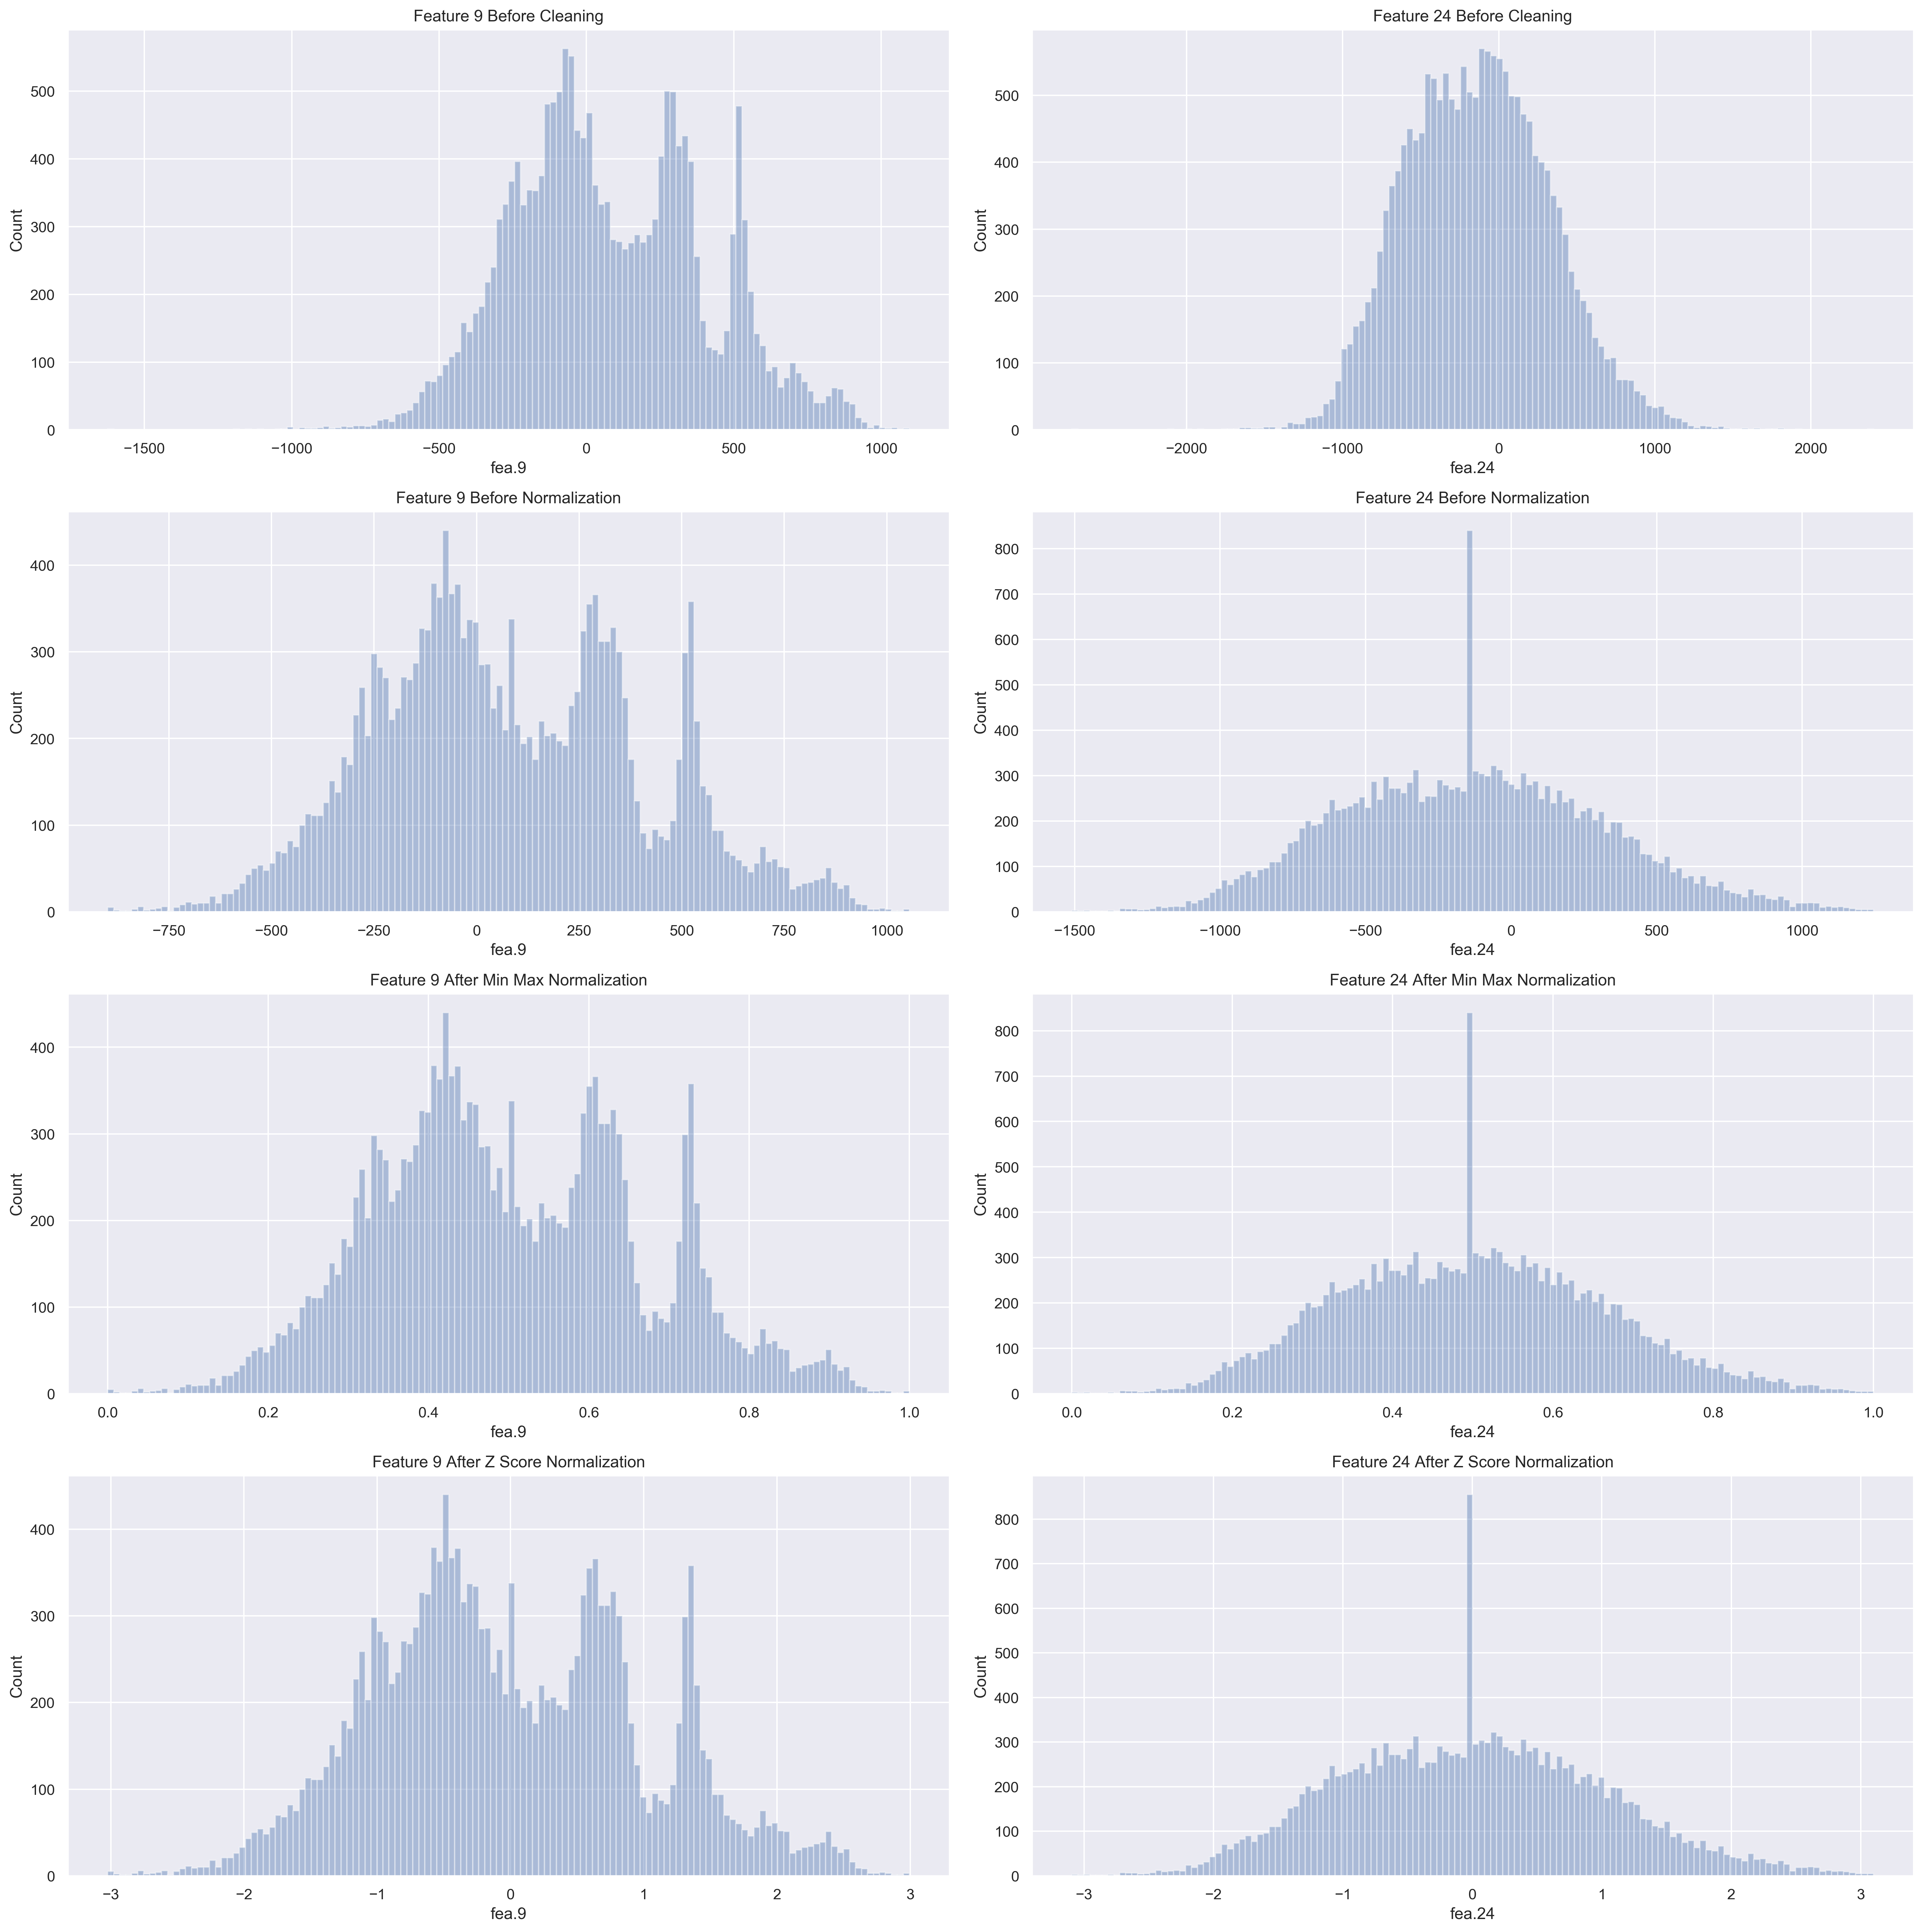
\includegraphics[width=6.1in]{assignment1/1-3-histograms.png}
\caption{\label{fig:fig1}histogram plots of feature 9 and 24 before and after normalization}
\end{figure}
